\documentclass[11pt]{article}
\usepackage[margin=1in]{geometry}
\usepackage{amsmath,amssymb,amsfonts}
\usepackage{graphicx,float}
\usepackage{fancyhdr,booktabs}
\usepackage{listings}
\usepackage{hyperref}
\lstset{
    language=Matlab,
    basicstyle=\ttfamily\small,
    breaklines=true,
    keepspaces=true,
    showstringspaces=false
}

% Header and Footer Setup
\pagestyle{fancy}
\fancyhf{}
\lhead{ME 351 -- Fall 2026}
\rhead{Homework 2}
\cfoot{\thepage}

\title{\textbf{ME 351}\\[0.5ex]\Large Homework 2}
\author{Zeshui Song}
\date{Fall 2026}

\begin{document}
\maketitle
\vspace{-1em}

For each sketch: mark open-loop poles with $\times$, zeros with $\circ$, show the real-axis portions of the locus, draw asymptotes when applicable, and indicate the direction of increasing $K$. A computer-generated root locus may be used to check your result after completing the hand sketch.

\subsection*{Exercise 1: Negative leading coefficient}
Consider
\[
1+KL(s)=0, \qquad K\geq 0,
\]
with
\[
L(s)=k_0\frac{\displaystyle\prod_{j=1}^{m}(s-z_j)}{\displaystyle\prod_{i=1}^{n}(s-p_i)}, \qquad k_0<0.
\]
Starting from the Evans phase condition and accounting explicitly for the phase contributed by $k_0$, derive the following three root-locus rules for $k_0<0$:
\begin{enumerate}
    \item[(a)] the pole--zero phase condition;
    \item[(b)] the rule determining which portions of the real axis belong to the root locus;
    \item[(c)] for relative degree $r=n-m>0$, the asymptote angles.
\end{enumerate}
State your final three rules clearly. Briefly explain why the branch start/end points and the centroid are unchanged by the sign of $k_0$.

\paragraph{Solution}\mbox{}\\
\textbf{Magnitude and phase conditions}\\
Starting from closed loop pole condition:
\[1+ K L(s) = 0 \implies K L(s) = -1\]
Thus, rewriting in phase and magnitude form for $K>0$:
\[K|L(s)| = |-1|=1 \quad \text{(magnitude)}\]
\[\angle KL(s) = \angle(-1) \quad \text{(phase)}\]
Note that the phase of a positive real number is $0$ or even multiples of $\pi$, and the phase of a negative real number is odd multiples of $\pi$, so it can be rewritten as:
\[\angle L(s) = (2\ell +1)\pi,\quad \ell\in\mathbb{Z}\]
Thus, a complex pole \(s\) is on the root locus if it satisfies the phase condition. For a pole \(s\) on the root locus, the corresponding gain \(K\) can be found by evaluating the loop transfer function at that point via the magnitude condition: $K = 1/|L(s)|$.\\\\
\textbf{Part (a): the pole-zero phase condition}\\
Defining the loop transfer function as a ratio of polynomials where $z_j$ are the zeros and $p_i$ are the poles, we have:
\[
L(s)=k_0\frac{\displaystyle\prod_{j=1}^{m}(s-z_j)}{\displaystyle\prod_{i=1}^{n}(s-p_i)}, \qquad k_0<0.
\]
Then the phase of the loop transfer function is:
\[\angle L(s) = \angle(k_0) + \sum_{j=1}^m \angle(s-z_j) - \sum_{i=1}^n \angle(s-p_i) = (2\ell +1)\pi,\quad \ell\in\mathbb{Z}\]
Note that multiplication corresponds to addition of angles, and division corresponds to subtraction of angles. Since $k_0<0$, we have $\angle(k_0) = \pi$. Thus, the phase condition can be rewritten as:
\[\angle L(s) = \pi + \sum_{j=1}^m \angle(s-z_j) - \sum_{i=1}^n \angle(s-p_i) = (2\ell +1)\pi,\quad \ell\in\mathbb{Z}\]
\[\boxed{\angle L(s) - \pi =  2\ell\pi,\quad \ell\in\mathbb{Z}\quad \text{(phase condition for negative $L(s)$)}}\]
\textbf{Part (b): Real axis segment condition}\\
Consider a test point $s_0$ on the real axis. The phase condition requires:
\[\angle L(s_0) = \pi + \sum_{j=1}^m \angle(s_0-z_j) - \sum_{i=1}^n \angle(s_0-p_i) = (2\ell+1)\pi,\quad \ell\in\mathbb{Z}\]
Thus, for any \textit{real} pole or zero, the phase contribution is either $0$ or $\pi$ depending on the sign (positive or negative) of the difference $s_0 - z_j$ or $s_0 - p_i$. 
\begin{itemize}
    \item If pole or zero is to the left of $s_0$, then $s_0 - z_j > 0$ or $s_0 - p_i > 0$, contributing $0$ to the phase.
    \[\angle (s_0 - p_i),\,\angle (s_0 - z_j) = 2\ell \pi,\quad \ell\in\mathbb{Z}\]
    \item If pole or zero is to the right of $s_0$, then $s_0 - z_j < 0$ or $s_0 - p_i < 0$, contributing $\pi$ to the phase.
    \[\angle (s_0 - p_i),\,\angle (s_0 - z_j) = (2\ell +1)\pi,\quad \ell\in\mathbb{Z}\]
\end{itemize}
Let $N_R$ be the number of real poles and zeros to the right of the test point $s_0$. Then the phase condition becomes:
\[\angle L(s_0) = \pi + N_R(2\ell +1)\pi = (2q+1)\pi,\quad \ell,q\in\mathbb{Z}\]
Simplifying gives a condition on $N_R$:
\[1 + N_R(2\ell +1) = 2q+1\]
\[N_R(2\ell +1) = 2q\]
\[N_R = \frac{2 q}{2\ell +1} \]
The numerator is even, and the denominator is odd. For an even integer divided by an odd integer, if the result is an integer, must be even. $\boxed{\text{Thus, $N_R$ must be even.}}$\\\\
\textbf{Part (c): Asymptotes}\\
Define the relative degree $r = n - m$ where $n$ is the number of poles and $m$ is the number of zeros.
\[
L(s)=k_0\frac{\displaystyle\prod_{j=1}^{m}(s-z_j)}{\displaystyle\prod_{i=1}^{n}(s-p_i)}, \qquad k_0<0.
\]
For $r>0$, when $|s| \to \infty$, the loop transfer function can be approximated as:
\[L(s) \approx k_0 \frac{s^m}{s^n} = k_0 s^{m-n} = k_0 s^{-r}\]
Write $s$ in polar form:
\[s = |s| e^{j\theta}\]
Plugging this into the approximation gives:
\[L(s) \approx k_0 |s|^{-r} e^{-j r \theta}\]
Since $k_0<0$, we have $\angle(k_0) = \pi$. Thus, the phase of the loop transfer function is:
\[\angle L(s) \approx \pi - r \theta\]
Apply the phase condition:
\[\angle L(s) \approx \pi - r \theta = (2\ell+1)\pi,\quad \ell\in\mathbb{Z}\]
Thus, the asymptote angles are:
\[\theta = - \frac{2\ell\pi}{r}\]
There are $r$ distinct asymptote angles, for values of $\ell > r$, the angles repeat (phase shifts by $2\pi$). Thus, the asymptote angles are (replace $\ell$ with $q$ to avoid confusion):
\[\boxed{\theta_q  = \frac{2q\pi}{r}, \quad q = 0, 1, \ldots, r-1}\]
\textbf{Why branch start/end points and the centroid are unchanged by $k_0$:}\\
The branch start and end points are determined by the locations of the open-loop poles and zeros, which are independent of the sign of $k_0$. Similarly, the centroid is determined only on the locations of the open-loop poles and zeros, and is given by:
\[
\alpha=\frac{\sum_{i=1}^{n}p_i-\sum_{j=1}^{m}z_j}{n-m}.
\]


\subsection*{Exercise 2: DC motor position control}
A simplified armature-controlled DC motor with position output can be modeled by
\[
P(s)=\frac{1}{s(s+2)}.
\]
With proportional position feedback $u=K(r-y)$, the loop transfer function is
\[
L(s)=\frac{1}{s(s+2)}.
\]
\begin{enumerate}
    \item[(a)] Sketch the complete root locus for $K\geq 0$. Determine the real-axis segments, asymptote angles, centroid, and the real-axis breakaway point.
    \item[(b)] Use the characteristic equation to determine the value of $K$ at the breakaway point.
    \item[(c)] As $K$ is increased beyond the breakaway point, what qualitative change occurs in the motor's closed-loop response? Explain from the pole locations.
\end{enumerate}

\paragraph{Solution}\mbox{}\\
\textbf{Part (a)}\\
Poles of $L(s)$:
\[s(s+2) = 0 \quad \implies s = 0, -2\]
Open loop zeros of $L(s)$: none\\\\
Relative degree:
\[r = n-m = 2-0 = 2\]
Centroid:
\[\alpha = \frac{\sum_{i=1}^{n}p_i-\sum_{j=1}^{m}z_j}{n-m} = \frac{(-2) - 0}{2-0} = -1\]
Asymptote angles:
\[\theta_q = \frac{(2q+1)\pi}{r}, \quad q = 0, 1\]
\[\theta_0 = \frac{\pi}{2}, \quad \theta_1 = \frac{3\pi}{2}\]
Real axis segments:
\[-2 \leq s \leq 0\]
Breakaway point:\\
This occurs when the two branches of the root locus meet on the real axis. The breakaway point can be found by solving for the repeated root of the characteristic equation. At a repeated root, both the derivative and the characteristic equation must be zero.
\[1 + C(s)P(s) = 0 \implies 1 + \frac{K}{s(s+2)} = 0\]
Rearranging gives:
\[s^2 + 2s + K = 0\]
Derivative with respect to $s$:
\[\frac{d}{ds}(s^2 + 2s + K) = 2s + 2 = 0 \implies s = -1\]
\begin{center}
    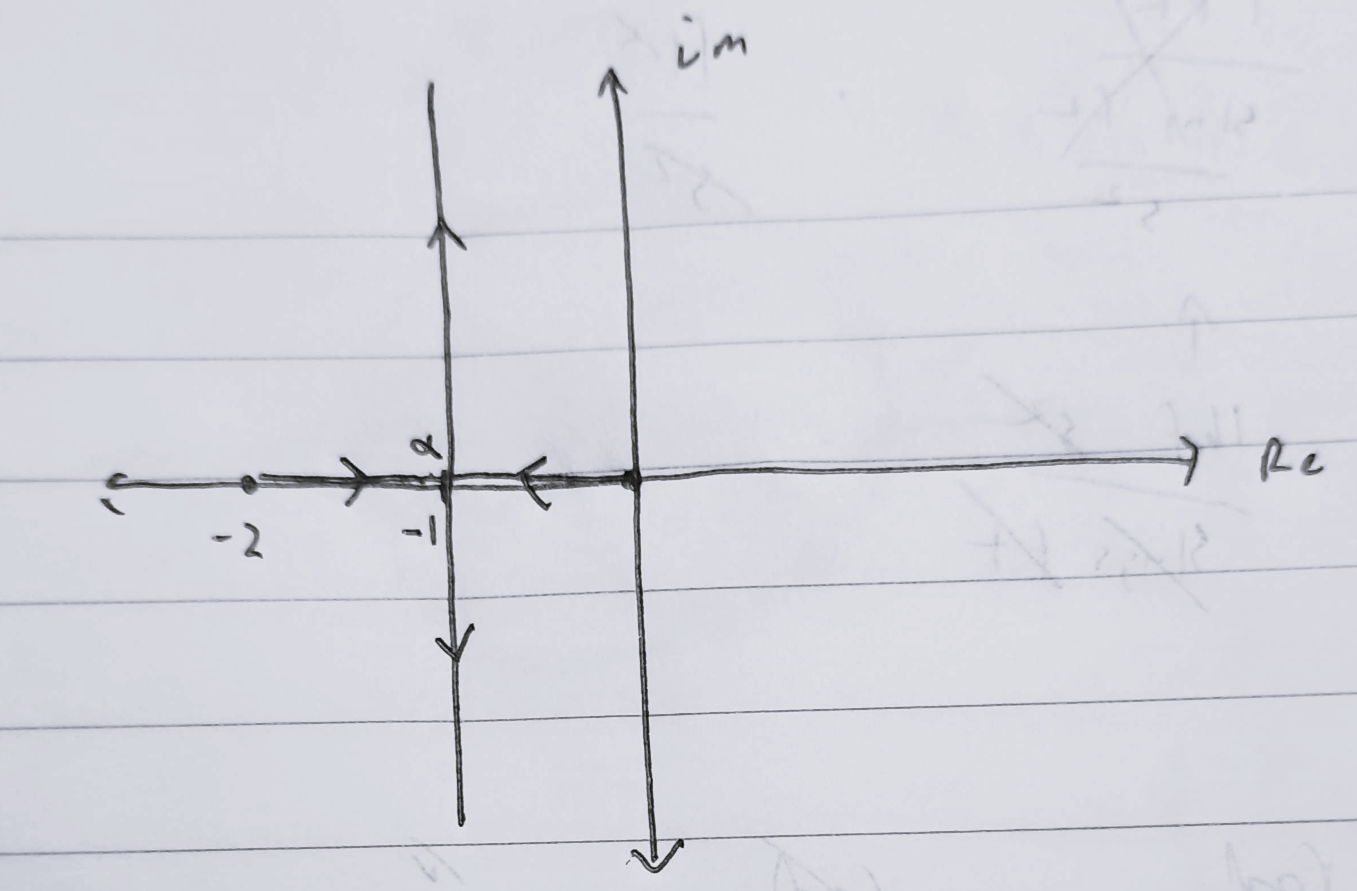
\includegraphics[width=0.5\textwidth]{P2 locus.png}
\end{center}
\textbf{Part (b)}\\
The gain at any point on the root locus can be found using the magnitude condition:
\[K = \frac{1}{|L(s)|}\]
Thus, at the breakaway point $s = -1$:
\[K = \frac{1}{|-1(-1+2)|} = \frac{1}{1} = 1\]
\textbf{Part (c)}\\
As $K$ is increased beyond the breakaway point, the closed loop response becomes oscillatory. This is because the poles move off the real axis and increases the imaginary part of the poles, which corresponds to increasing the frequency of oscillation. Since the real part of the poles is negative, the oscillations will decay over time.

\subsection*{Exercise 3: Flexible mechanical mode}
A lightly damped mechanical structure with force actuation and displacement sensing is approximated by
\[
P(s)=\frac{s+1}{s(s+2)(s+4)}.
\]
With proportional negative feedback, let
\[
L(s)=\frac{s+1}{s(s+2)(s+4)}.
\]
\begin{enumerate}
    \item[(a)] Sketch the root locus for $K\geq 0$. Identify the real-axis segments and the start and end points of all branches.
    \item[(b)] Determine the centroid and asymptote angles.
    \item[(c)] From your sketch, explain qualitatively what increasing feedback gain does to the dominant closed-loop poles. Is arbitrarily large gain obviously desirable?
\end{enumerate}

\paragraph{Solution}\mbox{}\\
\textbf{Part (a) + (b)}\\
Poles of $L(s)$:
\[s(s+2)(s+4) = 0 \quad \implies s = 0, -2, -4\]
Open loop zeros of $L(s)$:
\[s+1 = 0 \quad \implies s = -1\]
Relative degree:
\[r = n-m = 3-1 = 2\]
Centroid:
\[\alpha = \frac{\sum_{i=1}^{n}p_i-\sum_{j=1}^{m}z_j}{n-m} = \frac{(-2 + (-4)) - (-1)}{2} = -\frac{5}{2}\]
Asymptote angles:
\[\theta_q = \frac{(2q+1)\pi}{r}, \quad q = 0, 1\]
\[\theta_0 = \frac{\pi}{2}, \quad \theta_1 = \frac{3\pi}{2}\]
Real axis segments:
\[-1 \leq s \leq 0\]
\[-4 \leq s \leq -2\]
\begin{center}
    \includegraphics[width=0.5\textwidth]{P3 locus.png}
\end{center}
\textbf{Part (c)}\\
Increasing $K$ moves the pole at $s=0$ toward the zero at $s=-1$, give a faster decaying response. The other two poles at $s=-2$ and $s=-4$ move toward each other, eventually becoming oscillatory as imaginary components increase.\\\\
Thus, large gains are not obviously desirable, as the oscillatory response may be undesirable in some applications.
\subsection*{Exercise 4: A loop with $k_0<0$}
A sensor/actuator installation introduces an overall sign reversal in an otherwise stable first-order actuator and first-order plant. After writing the closed-loop characteristic equation in Evans form with $K\geq 0$, suppose the loop transfer function is
\[
L(s)=-\frac{s+1}{s(s+2)(s+4)}.
\]
Thus $k_0=-1$.
\begin{enumerate}
    \item[(a)] Using the rules you derived in Exercise 1, sketch the complete root locus for $K\geq 0$. Identify the real-axis segments, centroid, and asymptote angles.
    \item[(b)] Compare your sketch with Exercise 3. What changes when only the sign of $k_0$ is reversed, and what does not change?
    \item[(c)] Based on the root locus, determine whether increasing positive $K$ can destabilize this closed-loop system. Explain geometrically.
\end{enumerate}

\paragraph{Solution}\mbox{}\\
\textbf{Part (a)}\\
Poles of $L(s)$:
\[
s(s+2)(s+4) = 0 \quad \implies s = 0, -2, -4
\]
Open loop zeros of $L(s)$:
\[s+1 = 0 \quad \implies s = -1
\]
Relative degree:
\[r = n-m = 3-1 = 2\]
Centroid:
\[\alpha = \frac{\sum_{i=1}^{n}p_i-\sum_{j=1}^{m}z_j}{n-m} = \frac{(-2 + (-4)) - (-1)}{2} = -\frac{5}{2}\]
Asymptote angles:
\[\theta_q  = \frac{2q\pi}{r}, \quad q = 0, 1\]
\[\theta_0 = 0, \quad \theta_1 = \pi\]
Real axis segments: EVEN $N_R$\\
\[0 \leq s < \infty\]
\[-2 \leq s \leq -1\]
\[-\infty < s < -4\]
\begin{center}
    \includegraphics[width=0.5\textwidth]{P4 locus.png}
\end{center}
\textbf{Part (b)}\\
Both sketches have the same poles and zeros. However, the negative sign of $k_0$ changes the real axis segments and the asymptote angles. Instead, now all the poles stay on the real axis.\\\\
\textbf{Part (c)}\\
Increasing the gain $K$ does destabilize the system as the pole at $s=0$ moves to the right half plane.
\subsection*{Exercise 5: Verification}
Choose one of Exercises 2--4 and generate its root locus using MATLAB or the Python control package (for an example, see folder demos on MS Teams). Include the plot and briefly identify any feature of your hand construction that the numerical plot confirms (or corrects).

\paragraph{Solution}\mbox{}\\
\begin{center}
    \includegraphics[width=0.8\textwidth]{P5 verify.png}
\end{center}
This plot confirms the asymptotic behavior of the root locus as $K$ increases, as well as the real axis segments found using the revised rules for $k_0<0$.
\end{document}
